\documentclass{beamer}


\usepackage[frenchb]{babel}

\usepackage[T1]{fontenc}
%\usepackage[latin1]{inputenc}
\usepackage[utf8]{inputenc}

\usepackage{marvosym}



\newcommand{\be}[1]{ \begin{equation} \label{#1}}
\newcommand{\ee}{\end{equation}}


\newcommand{\bes}[1]{ \begin{equation} \label{#1}\begin{array}{rl}}
\newcommand{\ees}{\end{array}\end{equation}}


% \usetheme{default} -> A utiliser dans un premier temps

% \usetheme{Warsaw} -> A utiliser dans un second temps


\newcommand{\ssp}{\vspace{.2cm} }

\title{Approches globales, linéaires et non-linéaires, des instabilités hydrodynamiques.
}

\subtitle{"La stabilité globale pour les neuneus"}

\author{D. Fabre}

\institute{IMFT, groupe Interface}

\date{12 octobre 2017}


\begin{document}


\begin{frame}

\titlepage

\end{frame}

\section{Introduction}

\begin{frame}{Qu'es aquò ?? } 


Les problèmes d'instabilités sont omniprésents en mécanique des fluides. 

\ssp

Leur résolution fait appel à une classe de méthodes numériques spécifiques, 
complémentaires aux approches de simulation directe, qui sont actuellement en plein développement. 

\ssp


On parle {\em stabilité globale} quand la géométrie du problème necésssite une résolution en 2D (ou en 3D).

\ssp

(par opposition à {\em stabilité locale} quand des directions d'invariance (écoulement parallèle par ex.) permettent de rammener le problème à une résolution en 1D).


\end{frame}


\begin{frame}{Outils de résolution numérique}

Les méthodes d'éléments finis sont bien adaptés à ces problèmes.

Le logiciel {\em FreeFem++} est un outil très populaire dans la communauté de la stabilité hydrodynamique.

\ssp

%{\color{green} \Smiley{} \quad }  (solides, fluides, thermique, etc...)

{\color{green} \Smiley{} \quad } Syntaxe intuitive basée directement sur la formulation faible.

{\color{green} \Smiley{} \quad } Mailleur puissant et adaptatif (movemesh, adaptmesh, etc...)

{\color{red} \Frowny{} \quad } Interface graphique limitée (ffglut).

{\color{red} \Frowny{} \quad } Language interprété : pas adapté à la programmation fonctionnelle (mais des macros puissantes).
 
 \ssp

Necessité d'une surcouche "driver"  pour piloter les calculs et tracer les résultats en mode terminal ou par l'intermédiaire de sripts.
\ssp 
Choix : solveurs FreeFem / drivers Matlab.

\ssp -> Logiciel "Stabfem", développé à des fins d'enseignement et de recherche.


\ssp
{\color{orange}
\verb! https://github.com/erbafdavid/StabFem !
}

\end{frame}

\section{Linear stability }

\subsection{Step 0 : computation of a base flow}

\begin{frame}{Base flow}

We look for a steady base-flow $({\bf u}_b;p_b)$ satisfying the steady Navier-Stokes equations, i.e. 
$NS ({\bf u}_b,p_b) = 0$.


Suppose that we have a 'guess' for the base flow $[{\bf u}_b^g,p_b^g]$  which almost satisfies the equations.  We look for a better approximation under the form
\be{Newton1}
[{\bf u}_b,p_b]  = [{\bf u}_b^g,p_b^g] + [\delta {\bf u}_b, \delta p_b] = 0.
\ee

Injecting into the Navier-Stokes equation lead to $$
NS ({\bf u}_b^g,p_b^g) + NSL_{{\bf u}_b^g}(\delta {\bf u}_b,\delta p_b)$$


Where $NSL$ is the linearised Navier-Stokes operator. 
%defined by its action on a flow field $({\bf u} ; p)$ as follows 



=>  matricial problem with the form $A \cdot \delta X = Y$. The procedure of Newton iteration is to solve iteratively this set of equations up to convergence.

\end{frame}




\subsection{Eigenvalue computation}

\begin{frame}{Linear stability}

\be{startmodepropre}
{\bf u} = {\bf u}_b + \epsilon \hat{\bf u} e^{\lambda t} 
\ee

The eigenmodes is governed by the linear problem 
$$\lambda \hat{{\bf u}} = NSL_{{\bf u}_b}( \hat{\bf u},\hat{p})$$,

After discretization we end up with an eigenvalue problem with the matricial form
\be{Eigen_matricial}
\lambda B \hat{X} = A \hat{X}
\ee

\ssp
Iterative method : single-mode shift-invert iteration
$$
X^{n} =  (A- \lambda_{shift} B)^{-1} B X^{n-1}
$$ 

Generalization : Arnoldi

\end{frame}

\subsection{Adjoint problem} 

\begin{frame}{Adjoint problem}

\small

Define a scalar product :
$$
\left< \phi_1, \phi_2 \right> = \int_\Omega \overline{\phi_1} \cdot \phi_2   \mbox{ d} \Omega
$$


We can first define the {\em adjoint linearised Navier-Stokes operator} $NSL^\dag$ defined by the property:
\bes{NSLAdj}
\forall ( {\bf u}, p ; {\bf v}, q), & \left< NSL^\dag_{\bf U}( {\bf v},q) ,{\bf u}\right> + \left< \nabla \cdot {\bf v},p\right>  \\
=& \left< {\bf v}, NSL_{\bf U} ({\bf u},p)\right> + \left< q, \nabla \cdot {\bf u}\right>.
\ees
We can then define the adjoint eigenmodes as the solutions to the eigenvalue problem 
\be{EigenAdj} 
\forall ( {\bf u}, p), \quad  \lambda^\dag \left< \hat{\bf v}, {\bf u}\right> =
 \left< NSL^\dag_{\bf U}( \hat{\bf v},\hat{q}) ,{\bf u}\right> + \left< \nabla \cdot \hat{\bf v},p\right>  
\ee

Matricial form :

\be{Eigen_Adj_matricial}
\overline{\lambda}^\dag B \hat{X}\dag = A^T \hat{X}\dag.
\ee


\end{frame}

\begin{frame}{Adjoint mode and structural sensitivity}


Significance of the adjoint mode : 

(optimal perturbation)


\end{frame}




\section{Nonlinear global approaches to hydrodynamic instabilities}

\begin{frame}{Nonlinear global stability approaches : review}

%The linear stability approach approach is the right tool to predict instability threshold ($Re_c$) and the %shedding frequency at threshold ($St_c = \omega_c/2\pi$).

%\ssp
% But for $Re>Re_c$ it badly predicts the frequency of the limit cycle. 
 
$$
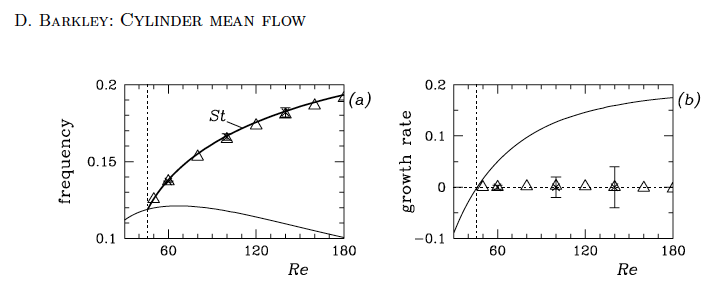
\includegraphics[width=8cm]{FIGURES/Barkley_figure.png}
$$

 
 
 \ssp It has been remarked that stability analysis of the {\em mean flow} obtained by time-averaging the limit cycle gives better predictions (Barkley, Leontini,...).
  
  
\ssp 
  
  => Objective of nonlinear stability approaches : Give a rigourous ground to study the stability of mean flow.
  
  

\end{frame}

\begin{frame}{Weakly nonlinear approach {\small (Sipp \& Lebedev, 2007)}}

Starting point : weakly non-linear expansion, with multiple scale method.

$$
\epsilon : \frac{1}{Re_c} - \frac{1}{Re} ; \quad \tau = \epsilon^2 t
$$

\begin{eqnarray}
{\bf u} &=& {\bf u}_{bc} + \epsilon \left[ A_{wnl} (\tau) \hat{\bf u} e^{i \omega_c t} + c.c. \right] \label{WNL1}\\
&+& \epsilon^2 \left[ {\bf u}_\epsilon + |A_{wnl}|^2  {\bf u}_{2,0} + \left(  A_{wnl}^2 {\bf u}_{2,2} e^{2 i \omega_c t} + c.c. \right) \right] + {\cal O}( \epsilon ^3)
\nonumber
\end{eqnarray}


\end{frame}



\begin{frame}{Self-Consistent approach {\small (Mantic-Lugo, Arratia \& Gallaire, 2014)}}

Starting point : Pseudo-eigenmode decomposition



\end{frame}


\begin{frame}{Harmonic-Balance}

\end{frame}




\end{document}

